\documentclass[french]{article}

\usepackage{geometry}
 \geometry{
 a4paper,
 total={150mm,240mm},
 left=30mm,
 top=30mm,
 }


\usepackage{helvet}

\usepackage[utf8]{inputenc}
\usepackage[T1]{fontenc}
\usepackage[french]{babel}
\usepackage{comment}
\usepackage{subcaption}
\usepackage{subfiles}
\usepackage{graphicx}
\usepackage{diagbox}
\usepackage[table,xcdraw]{xcolor}
% \usepackage{minted}
\usepackage{placeins}

\usepackage{fancyhdr}



\graphicspath{ {./img/} }

\title{\fontfamily{phv}\selectfont \Huge \textbf{Panic At Tortuga}}
\author{\fontfamily{phv}\Huge{Rapport de projet}}
\date{\fontfamily{phv}\selectfont Juin 2021}

\begin{document}

\begin{titlepage}
    \maketitle
    
    \thispagestyle{empty}
    % {\fontencoding{T1}\fontfamily{calligra}\selectfont the font is temporarily changed}
    \vspace{10pt}
    \begin{figure}[hbt!]
        \centering
        
\includegraphics[scale=0.43]{logo.png}
    \end{figure}
    \vspace{10pt}

    \begin{figure}[hbt!]
        \centering
        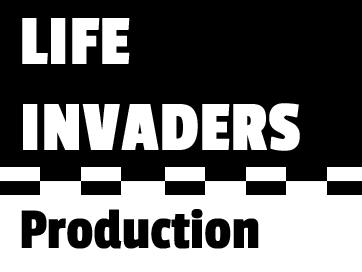
\includegraphics[scale=0.84]{logo_lifeinvaders_copie.png}
    \end{figure}
\end{titlepage}

% ////////////////////////////////////////////////
% ////////////////////////////////////////////////
% ////////////////////////////////////////////////


\tableofcontents
\newpage

\pagestyle{fancy}
\lhead{Panic At Tortuga}
\fancyhead[C]{Avril 2021}
\rhead{LifeInvaders Production}

\section{Introduction}

% introduction à compléter
L'heure du rendu final a sonné. Cette dernière période de travail n'a pas été la plus calme, car rythmée par un TD de maths et les partiels de fin d'année.
Cependant, le projet n'a pas cessé d'évoluer pour atteindre sa forme finale, plutôt aboutie.

\newpage
\section{Présentation}
\subfile{sections/presentation.tex}
\section{Développement}
\subfile{sections/timeline.tex}
\subfile{sections/progression.tex}
\subfile{sections/launcher.tex}
\subfile{sections/ia.tex}
\subfile{sections/map.tex}
\subfile{sections/ui.tex}
\subfile{sections/website.tex}
\subfile{sections/multiplayer.tex}
\subfile{sections/gameplay.tex}
\subfile{sections/graphismes.tex}
\subfile{sections/prev.tex}
\subfile{sections/bibliographie.tex}
\newpage
\section{Conclusion}
% conclusion à changer
Le projet Panic at Tortuga aura été un réel défi technique, et nous aura demandé beaucoup d'investissement pour arriver à sa forme finale. Tous les éléments, 
des mécaniques de jeu au multijoueur, auront représenté des dizaines d'heures de travail, pendant lesquelles nous avons gagné en compétences et appris à utiliser 
Unity, ce que nous serons peut-être amenés à refaire dans notre vie professionelle. Certaines tâches, comme la carte, nous auront enseigné la patience, et d'autres 
comme la synchronisation Photon, nous auront appris à nous dépasser. Les rapports de soutenance, par la régularité qu'ils imposent, ont permis un avancement 
constant du jeu, sans périodes d'inactivité prolongée. 
\listoffigures
\listoftables
\end{document}
